\chapter{Analysis}
In this chapter, we describe a method to automatic extraction landmarks from biological images. The process includes some steps as follows:
\begin{enumerate}
\item Segmentation (includes preprocessing image and extracting the features),
\item Construction and comparison the Pairwise Geometric Histogram,
\item Estimation the global pose of object by the Probabilistic Hough Transform,
\item Refinement the estimated landmarks by template matching.
\end{enumerate}
\section{Segmentation}
Segmentation is a process to extract interested features (lines) from the digital image. The expected result in this process is the list of the approximate lines which are used to construct the pairwise geometric histogram. \\[0.2cm]
The process mainly separate into two stages: firstly, we pre-process image; secondly, we extract the image's features. In first stage, we reduce the noise as well as enhance the quality of image. In second stage, we extract the features based on the edge segmentation. After that, by applying the appropriate technique to obtain the step edges and broken the edges into approximate lines.
\subsection{Pre-process image}
Pre-processing is a process that reduces the noises of image and enhance the quality of image's features. To do that, the simplest method in segmentation was used, \textbf{threshold}. When we apply \textbf{threshold} method, the \textit{threshold value} is important in this technique. Usually, the threshold value might indicated follows two ways: manually or automatically. In the concept of this report, we will introduce a method to indicate the threshold value by analysing the image histogram. This method will be focused in next chapter.
\begin{figure}[h!]
\centering
\subfloat[Image with noise]{\label{fig:seg_211}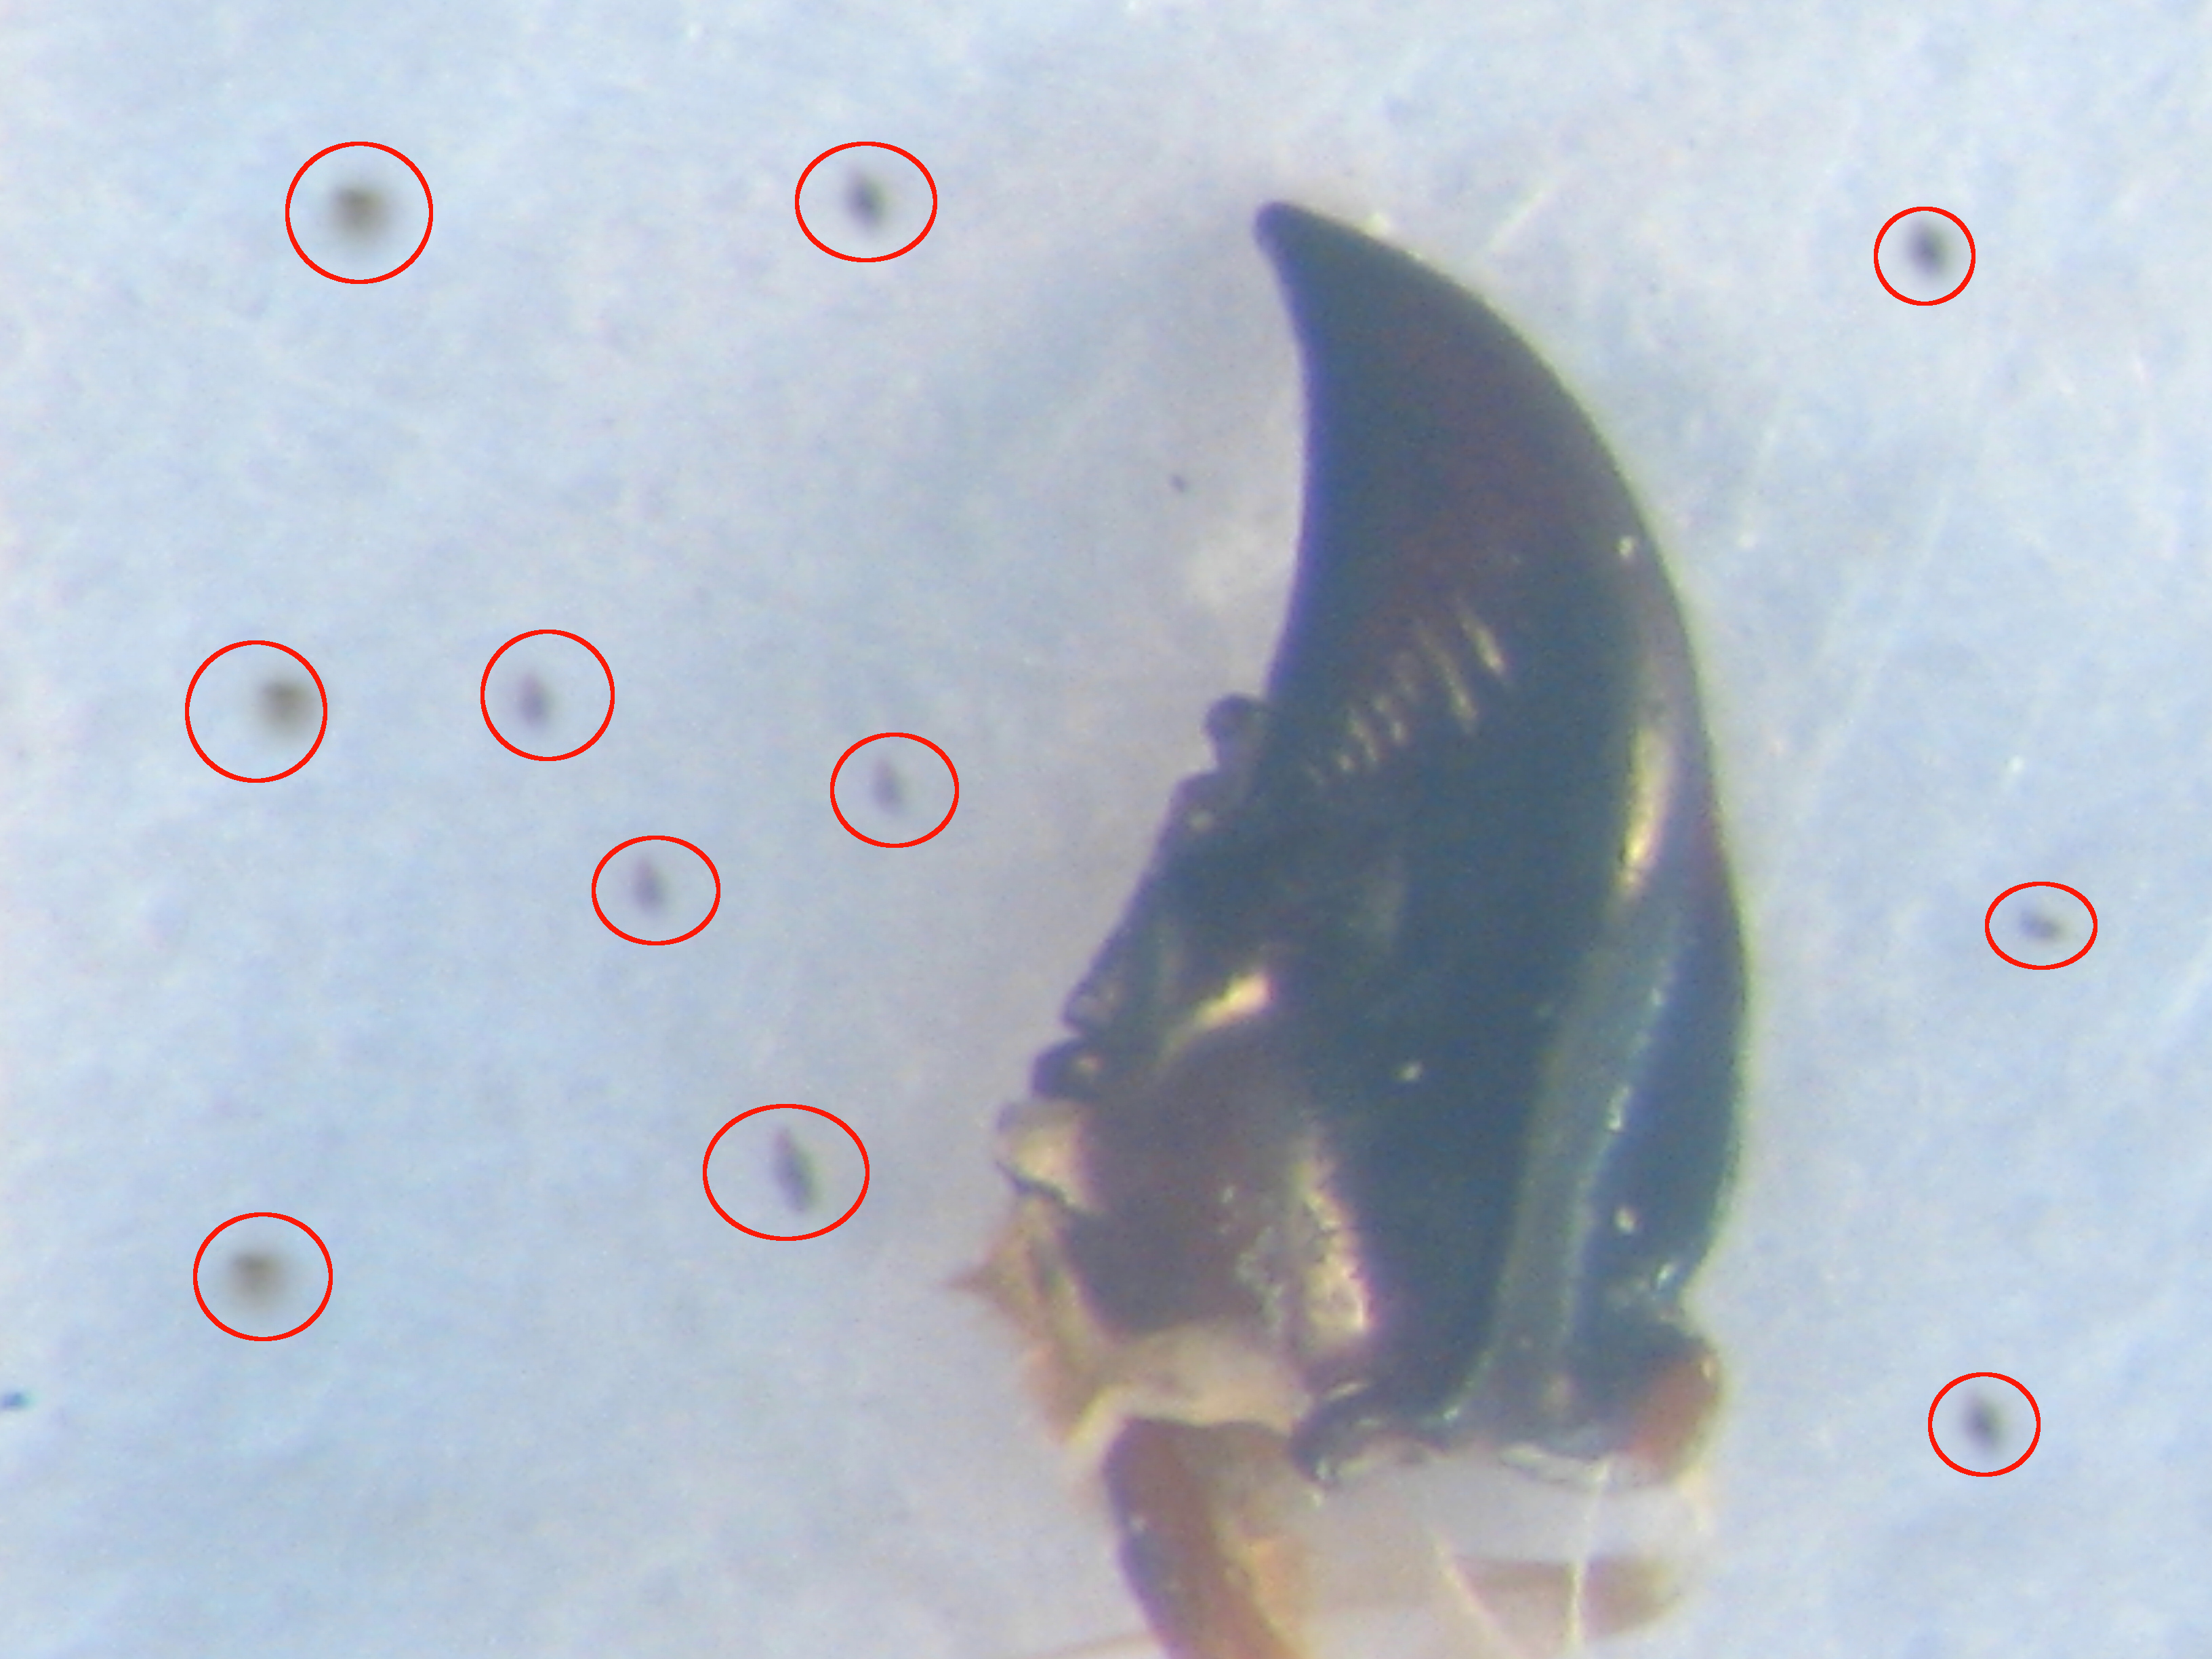
\includegraphics[width=0.45\textwidth]{./images/md019n}}~~
\subfloat[Image without noises]{\label{fig:seg_212}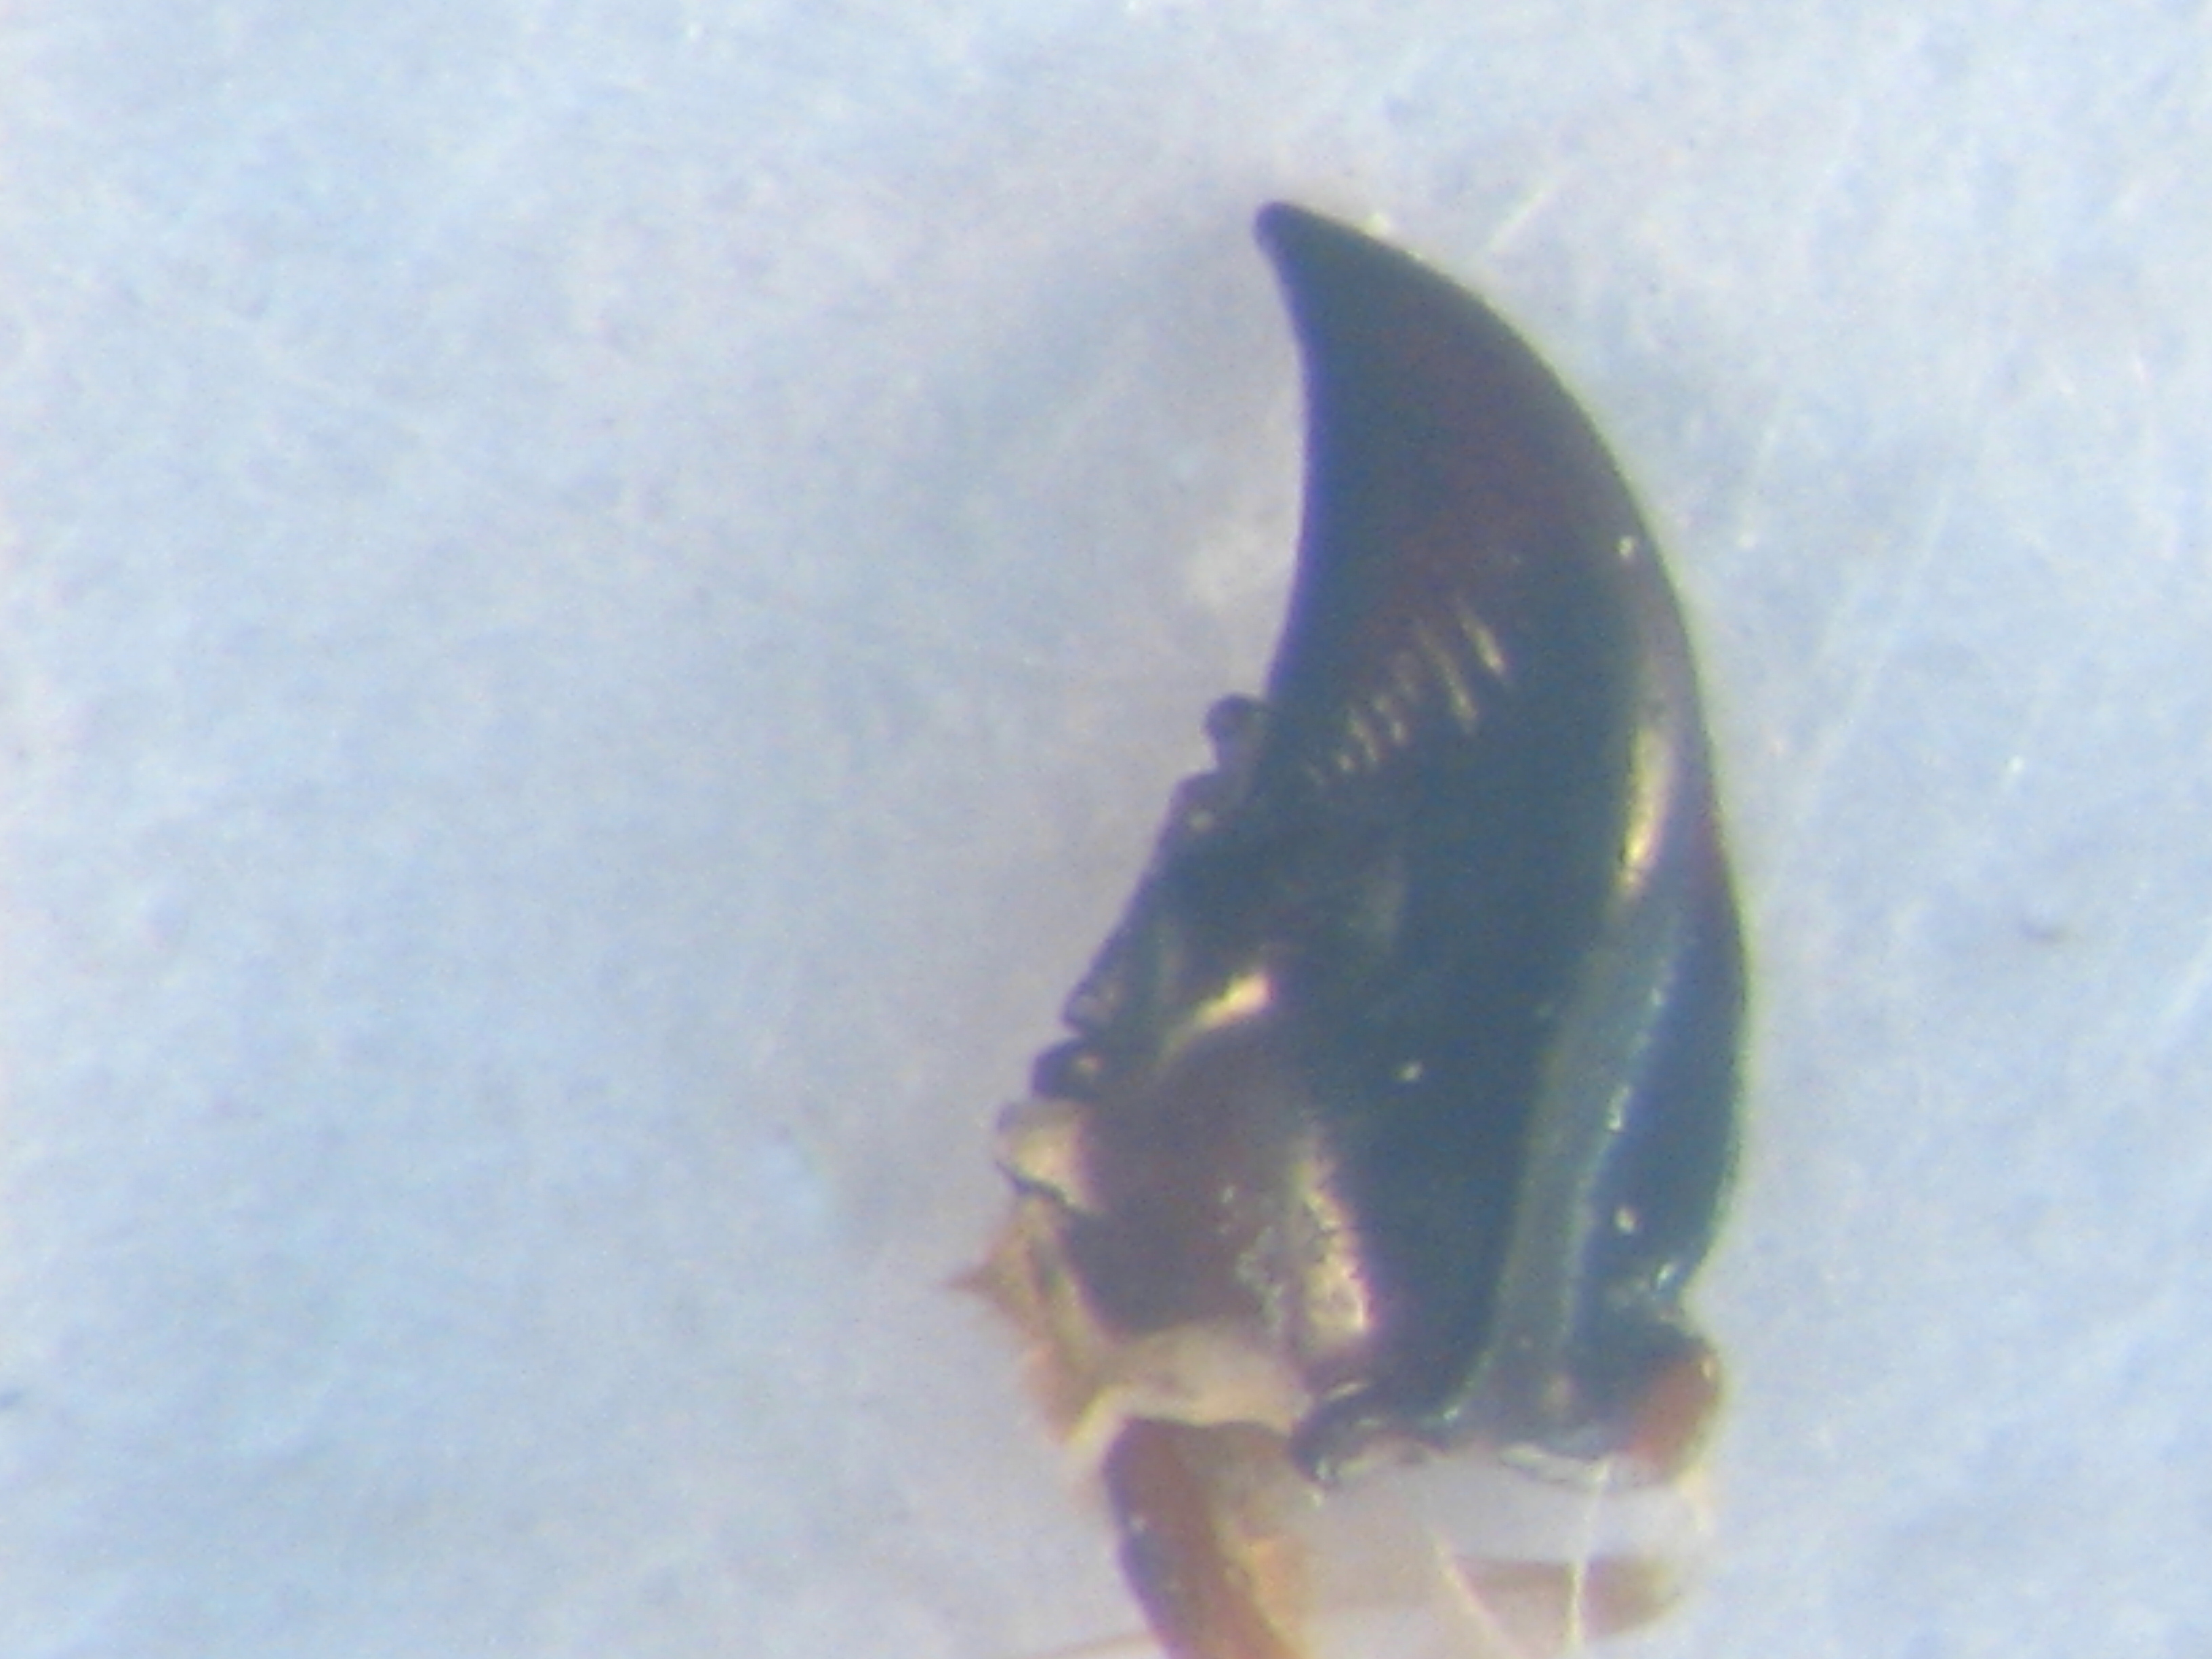
\includegraphics[width=0.45\textwidth]{./images/md019no}}
\caption{Example about noises in image}
\label{fig:figure_21}
\end{figure}
\subsection{Feature extraction}
After reducing the noise from input image in pre-processing step. In this step, by applying suitable technique, we can extract the interested in features (edges) from the image. The Canny\cite{canny1986computational} algorithm, which incorporates non-maximal suppression and hysteresis thresholding, is used to detect the step edges. In Canny algorithm, the important parameters are the two threshold values (\textit{lower threshold} and \textit{upper threshold}) and the aperture size of the Sobel operator, it decides the pixels kept. Normally, the value of lower threshold and upper threshold follows a certain rate. The inputs which we need to know when applying the Canny algorithm as follows:
\begin{itemize}
\item \textit{Source}: the input image (in grayscale mode)
\item \textit{Destination}: the output image,
\item \textit{Lower threshold}: the first (lower) threshold value,
\item \textit{Upper threshold}: the second (upper) threshold value,
\item \textit{Kernel size}: size of kernel, aperture for the Sobel operator.
\end{itemize}
The Canny algorithm is not aware of the actual edges, the edge detecting process was based on the Sobel operator, extracted with non-maximal suppression. To obtain the expecting result, we need to apply another technique to obtain the step edges. In this case, we can use the technique to analysis the structure of topology to get the edges. This technique was proposed by Suzuki\cite{suzuki1985topological}.
\subsection{Edge segmentation}
The geometric relation could not be constructed from the edges, it is always constructed from the relation of basic geometric objects, such as the lines.  In fact, any arbitrary edge can be represented by a set approximate lines. Instead an edge, we represent a set of approximate lines of it. This method is useful when we want to present the edges or describe the relationship between the edges in an object. From the set of step edges was obtained from find contours (the image structure), in this step, we will segment each step edge into approximated lines. The method to segment the edges is the recursive algorithm\cite{thacker1995assessing}. The last result of this step is a set of approximate lines with the edges of image. These will used to describe the shape in the compact invariant at next stage. An example about edge segmentation is presented in figure \ref{fig:figure_22}.
\begin{figure}[h!]
\centering
\subfloat[Original image]{\label{fig:seg_221}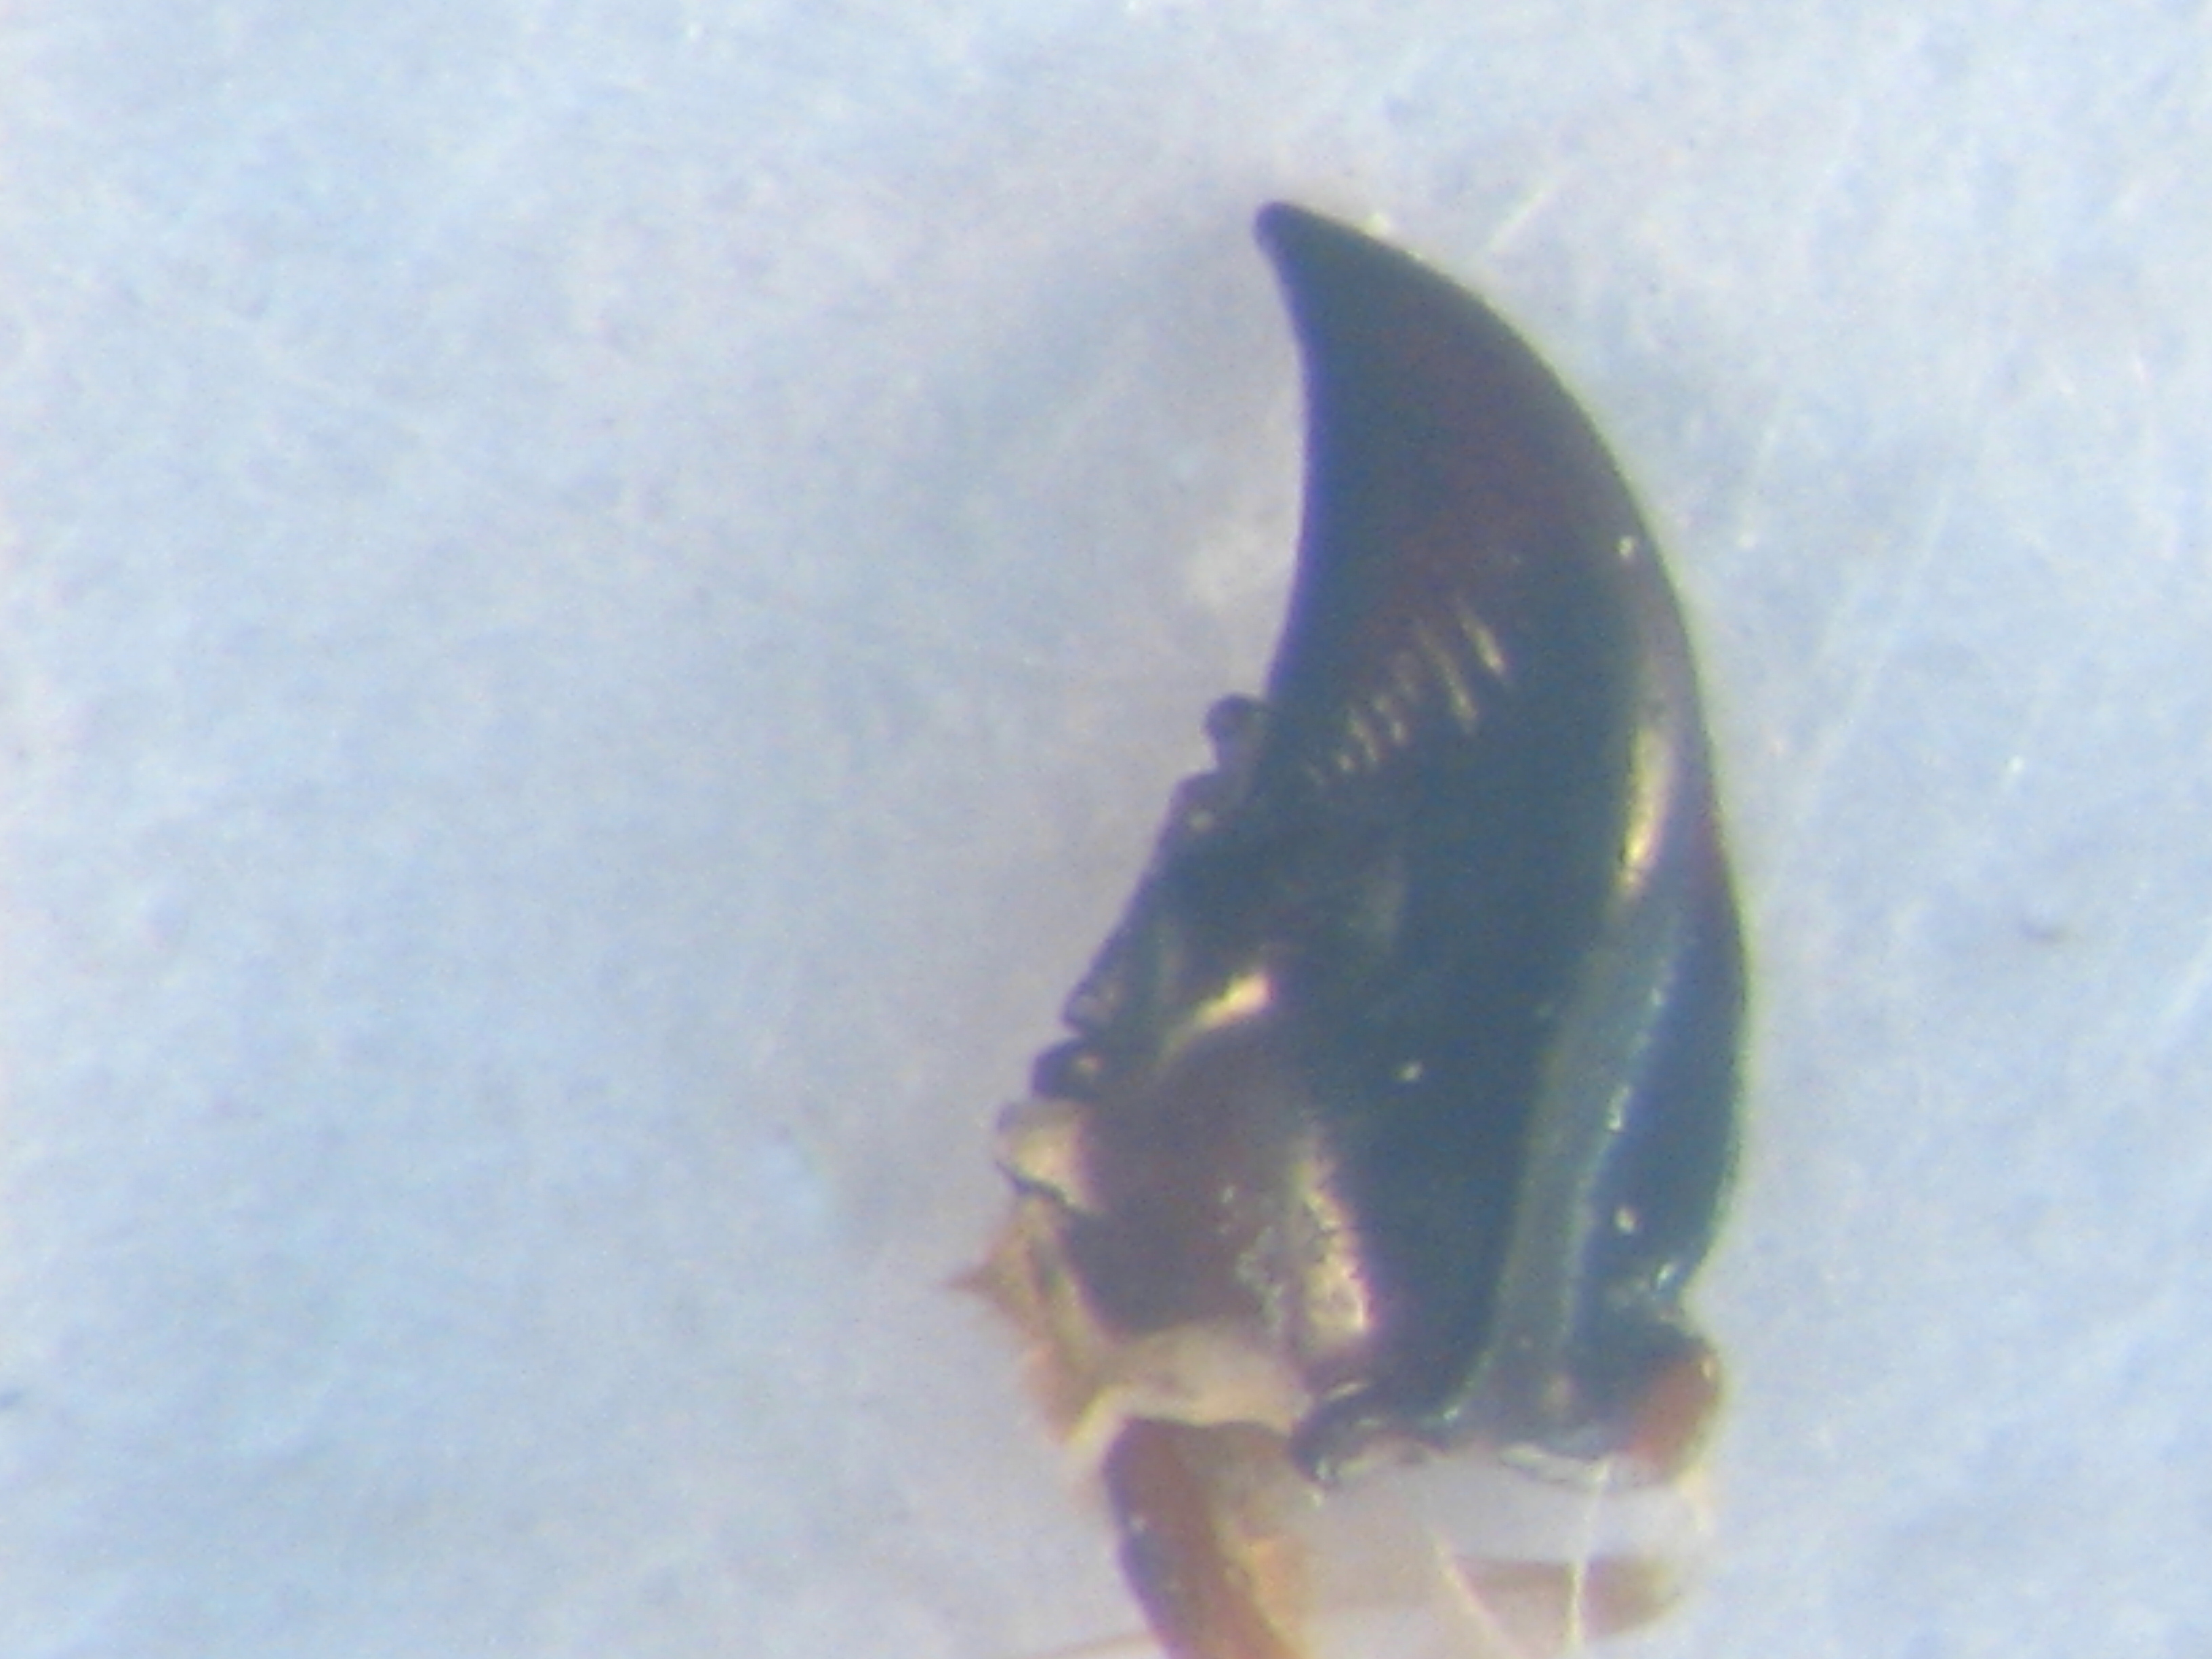
\includegraphics[width=0.45\textwidth]{./images/md019no}}~~
\subfloat[Image with line segmentation]{\label{fig:seg_222}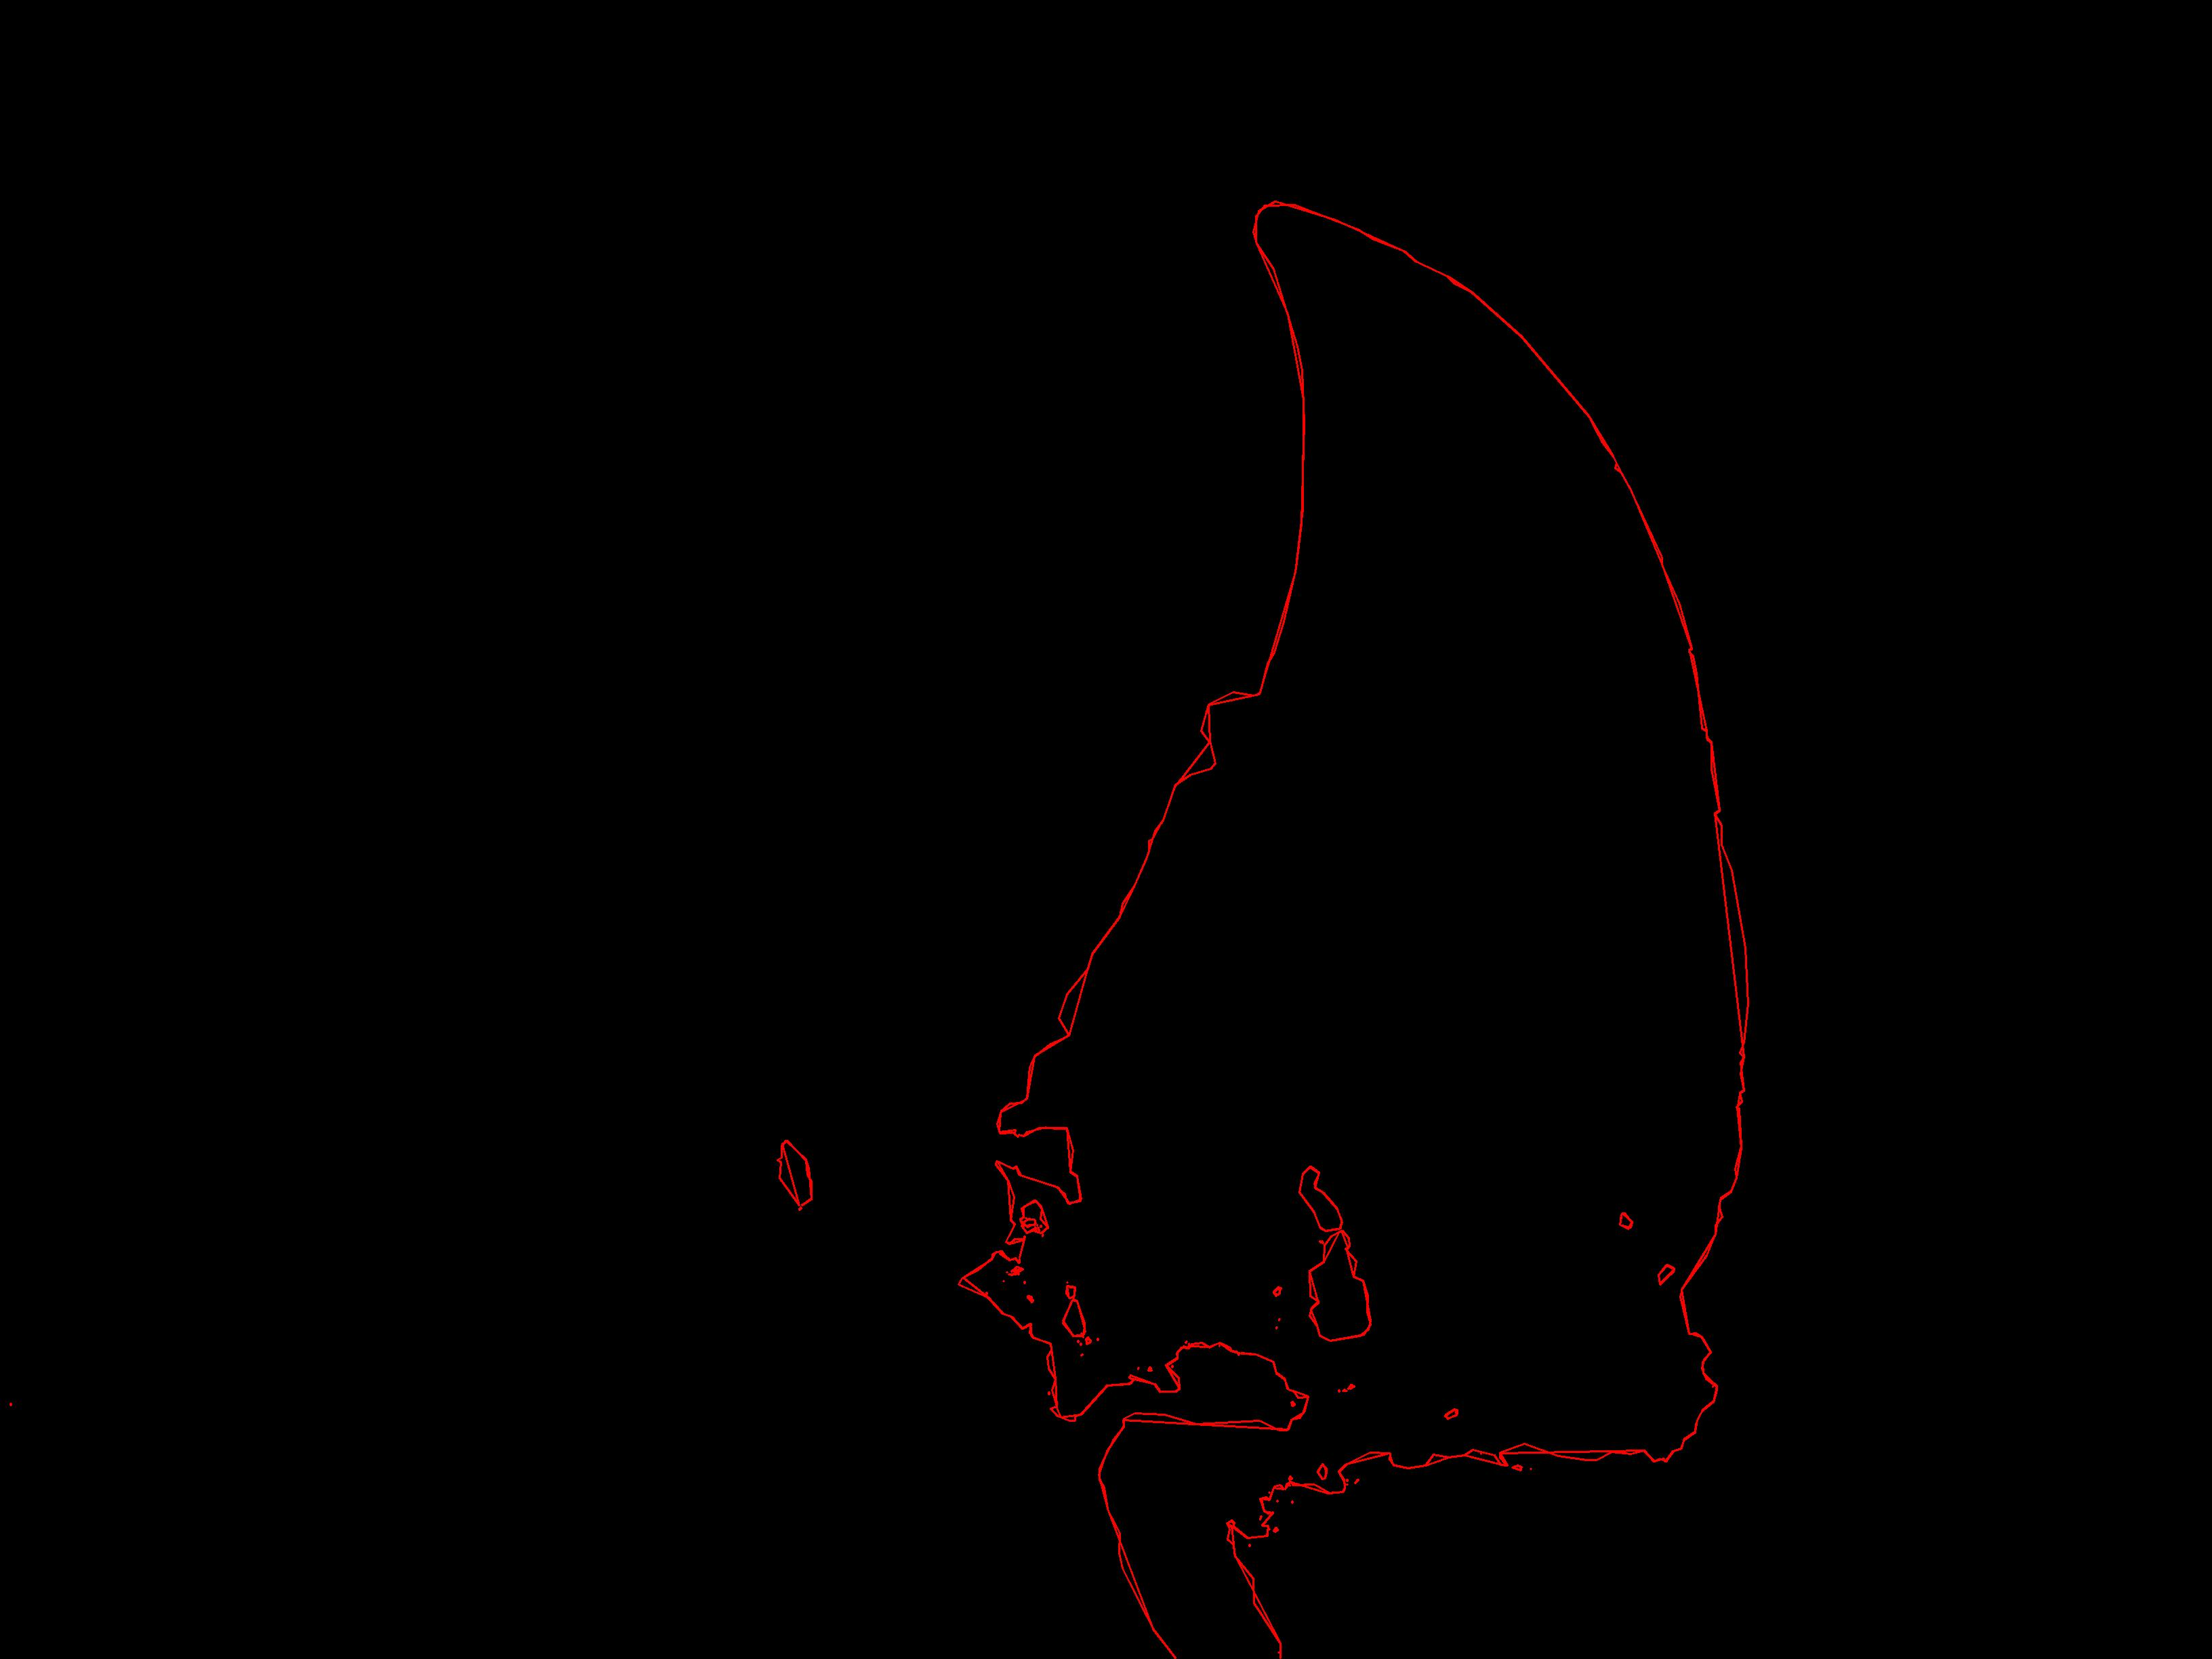
\includegraphics[width=0.45\textwidth]{./images/md019seg1}}
\caption{An example about image segmentation}
\label{fig:figure_22}
\end{figure}
\section{Pairwise Geometric Histogram}
Pairwise Geometric Histogram(PGH)\cite{evans1993use} is used to encode the relative information between a line and a set of lines in an object. Therefore, an object can be represented by a set of PGH. From the set of PGH, we can reconstructed the object or compare to another object. In this section, we introduce the construction of a PGH for an object based on the geometrical relationship and compute the similar distance between two objects.\\
The PGH is constructed on the geometric features between lines relative. The geometric features are characteristic which can describe the geometric shape such as angle, the length of line, perpendicular between two lines, etc. For the shape representation, the relative angle and perpendicular distance is geometrical features useful.\\
\begin{figure}[h!]
\centering
\subfloat[The geometric relationship between two lines]{\label{fig:231}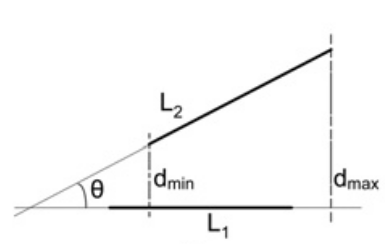
\includegraphics[width=0.4\textwidth]{./images/PGH_geo}}~~
\subfloat[The pairwise geometric histogram ]{\label{fig:232}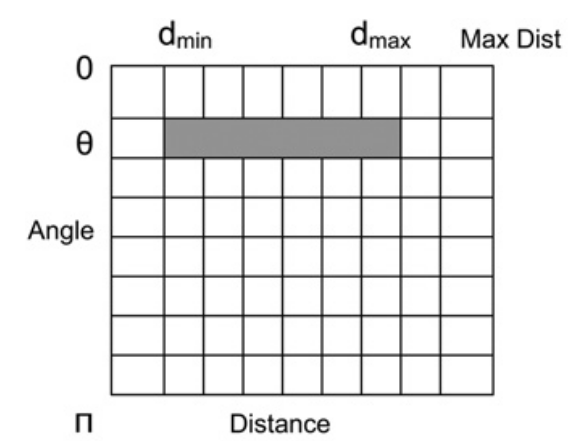
\includegraphics[width=0.4\textwidth]{./images/PGH}}
\caption{Example about geometric features and the pairwise geometric histogram}
\label{fig:figure_23}
\end{figure}
As example in figure \ref{fig:figure_23}, the figure \ref{fig:231} represents the geometric relationship between two lines \textbf{L1, L2}. The figure \ref{fig:232} represents the PGH between them when using line \textbf{L1} as reference line and line \textbf{L2} as object line.
\subsection{Local pairwise geometric histogram}
The local PGH presented the relationship between a reference line with other lines of shape. Thus, for each line in object, we can construct a local PGH for it. The frequency of the geometric features is recorded as a two dimensional histogram with an angle axis and distance axis. The entries on PGH describes the geometric relationship between the reference line and the object lines. The blurring of entry along the axis regarding the true position and orientation of each object lines for reference line. Following the accuracy, we can indicate the size of histogram and normalize the value to match with size of histogram.
\subsection{Global pairwise geometric histogram}
Based on local PGH constructor, global PGH is combined of all local PGHs of all lines belong to the object. It means if the object is defined by n lines, the global PGH will composed of n local PGHs. This method is good when we apply some variants on the image, such as translate or rotate the image because the angle and perpendicular distance between a pair of lines are invariant.
\subsection{Histogram matching}
\textbf{``The histogram matching enables robust classification of shape features by finding similarity between the scene and reference model"}\cite{palaniswamy2010automatic}. The similar between two models can obtain via the similar distance, which is computed by comparing their probability distribution on geometric histogram. To solve it, each model is represented by a global PGH and uses the Bhattacharya\cite{thacker1995assessing} metric to determine the similar distance between the two models \cite{palaniswamy2010automatic}. In general, we can be normalize the histograms before comparing. The form of Bhattacharrya metric used to compute the similarities between two models is:
\begin{center}
\begin{equation} \label{eq:1}
d_{Bhattacharyya} (H_{i}H_{j}) = \sum\limits_{\theta}^{\pi}\sum\limits_{d}^{d_{max}}\sqrt{H_{i}(\theta,d)H_{j}(\theta,d)}
\end{equation}
\end{center}
The significance of parameters in the formula \ref{eq:1}, as follows:
\begin{itemize}
\item $\theta$: angle value, range of $\theta$ in angle axis from 0 to $\pi$.
\item $d$: the perpendicular distance, range of d in perpendicular distance from 0 to the maximum distance of arbitrary lines of shape.
\item $H_{i}(\theta,d)$ is an entry at row $\theta$ and column d in histogram of image \textit{i}
\item $H_{j}(\theta,d)$ is an entry at row $\theta$ and column d in histogram of image \textit{j}
\end{itemize}
\section{Probabilistic Hough Transform}
\textbf{Hough transform} is a technique used to extract the features in images. The main idea of this method based on the vote procedure to find the best similar of object in a certain class of objects. The Hough transform was originally developed to recognize the line\cite{hough1962method} and after, it has extended to apply on arbitrary shape\cite{duda1972use}.\\[0.2cm]
The \textbf{generalised Hough transform}\cite{ballard1981generalizing} (GHT) is the modification of Hough transform. It can used to detect an object described with its model. The problem solved with GHT is finding the model's position in the image. Like \textbf{Hough transform}, GHT also use on the vote procedure to solve the problem. Following the similarity metric (by Bhattacharya), the hypothesised matches can used as input in pose estimation algorithm such as the generalised Hough transform. But in this case, it do not apply. Instead, the probabilistic Hough transform (PHT) is used to estimate the global pose of shape\cite{ashbrook1995robust}.\\[0.3cm]
Based on a group of features within the scene image, identifying the represent of a model image in a scene image. The hypothesised location of the model image in the scene image is indicated based on the conditional probability that any pair scene lines agreement about a position in model image.\\[0.3cm]
Estimating the global shape has two main steps. Firstly, training process starts with recording the perpendicular distance and the angle from a reference point to each pair of model lines, then finding the similar pairs between model image and scene image. Secondly, estimating process starts as predicting the pose of scene image different from the model image, then we estimate the location of the model landmarks on scene image.
\subsection{Training process}
Training process is process recording the relationship of model to a reference point in model. The reference point can be chosen at arbitrary position on the model image. At this step, the perpendicular distance and angle from each pair model lines to a reference point was recording and saving (called reference table). The expected result in this process is similar pairs between model image and scene image. At this step, PHT used to do that. The chosen pair of scene lines obtained from best votes when we consider the similarity between each pair of scene image and model image.
\subsection{Estimating process}
The estimating process is duration that estimating the reference landmarks on the scene image. Firstly, we estimate the position of model's reference point on scene image. Secondly, we estimate the model's reference landmarks on the scene image from the position of model's reference point in the scene image. With a pair of scene lines agree with a pair of model lines was chosen at previous step, the model's reference point in the scene image can be detected by extending the perpendicular lines of the pair of scene lines at the appropriate position.\\[0.2cm]
The estimation of model's landmarks in the scene image can be estimated by calculating the relatedness between the model's reference point and the model's landmarks. Besides, we also record the difference about rotation, orientation and scale between the model image and the scene image.
\begin{figure}[h!]
\centering
\subfloat[The model image]{\label{fig:241}
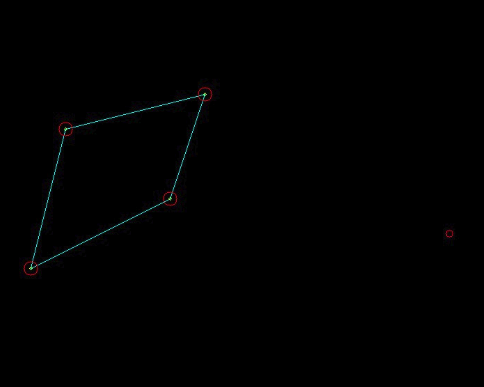
\includegraphics[width=0.4\textwidth]{./images/pht_1}}~~
\subfloat[The scene image ]{\label{fig:242}
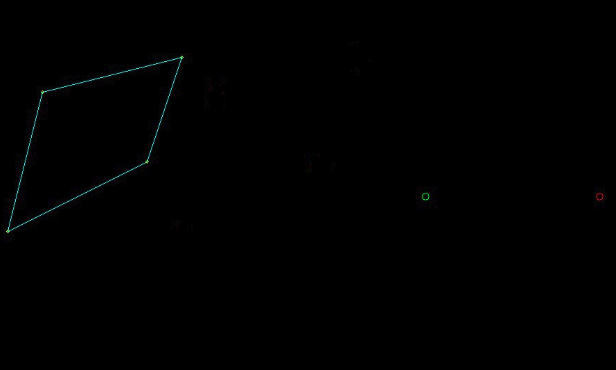
\includegraphics[width=0.4\textwidth]{./images/pht_2}}
\caption{The landmarks estimated by probabilistic Hough transform}
\label{fig:24}
\end{figure}~\\
In figure \ref{fig:24}, we apply the PHT to estimate the landmarks of the model to the scene. The image in figure \ref{fig:241} as the model. In the model, the small red circle and large red circles are the reference point and the landmarks in model, respectively. The image in figure \ref{fig:242} as scene. By applying the PHT, we estimate the reference point (green circle) in the scene and the location of the landmarks (the yellow circles).
\section{Template matching}
Template matching is the process to refine the estimated landmarks, which was obtained by PHT of the scene image with an appropriate method. In the scope of this method, we use the cross-correlation to refine the estimated landmarks from PHT stage.\\[0.2cm]
Cross-correlation is a method of estimating the similarity between the two signals. By computing the sum of products between two signals when a signal is sliding on another signal. The position is considered similarity if the value at this position is maximal. Cross-correlation is used for searching a short signal in a longer signal. In image processing, it used to detect the present of an object (template) in a large object (image). The equation of cross-correlation is as follows (equation \ref{eq:cross-correlation}):
\begin{center}
\begin{equation}\label{eq:cross-correlation}
R_{ccorr}(x,y) = \sum\limits_{x',y'}[T(x'.y').I(x + x', y + y')]
\end{equation}
\end{center}
Where:
\begin{itemize}
\item T is template which use to slide and find the exist in other image.
\item I is image which we expect to find the template image
\item $(x', y')$ are coordinates in template where we get the value to compute.
\item $(x + x', y + y')$ are coordinates in image where we get the value to compute when template $T$ sliding.
\end{itemize}
By sliding the template on image by each pixel from left to right and top to down. At each position, we compute the $R_{ccorr}(x,y)$. The position have maximal $R_{ccorr}(x,y)$ is positioned that best similar of template in image.\\[0.2cm]
However, if we use the original image to compute and find the similarity, the brightness of the template and the image might change the conditions and the result. So, we can normalize the image before applying the cross-correlation to reduce the effect of lighting difference between them. The normalization coefficient is:
\begin{center}
\begin{equation}\label{eq:normalizeCoff}
Z(x,y) = \sqrt{\sum\limits_{x',y'}T(x'.y')^{2}.\sum\limits_{x',y'}I(x + x', y + y')^{2}}
\end{equation}
\end{center}
The value of this method when we normalized computation as below:
\begin{center}
\begin{equation}\label{eq:cross-correlation}
R_{ccorr\_norm}(x,y) =\frac{R_{ccorr}(x,y)}{Z(x,y)} = \frac{\sum\limits_{x',y'}[T(x'.y').I(x + x', y + y')]}{\sqrt{\sum\limits_{x',y'}T(x'.y')^{2}.\sum\limits_{x',y'}I(x + x', y + y')^{2}}}
\end{equation}
\end{center}
